
%
% Beispieldokument für TU beamer theme
%
% v1.0: 12.10.2014
% 
\documentclass[xcolor={dvipsnames}]{beamer}
\usetheme{TU}

\usepackage{booktabs}
\usepackage{tabularx}
% Macro to make entire row bold from https://tex.stackexchange.com/questions/309833/format-whole-row-of-table-as-bold
\newcommand\setrow[1]{\gdef\rowmac{#1}#1\ignorespaces}
\newcommand\clearrow{\global\let\rowmac\relax}
\clearrow

\title{Online Learning Per-flow Queuing Policies}

%\author[M. Bachl et al.]{%
%	\underline{Maximilian Bachl}\email{maximilian.bachl@tuwien.ac.at} \and Fares Meghdouri \and Tanja Zseby \and Joachim Fabini
%}
\author[M. Bachl]{%
	Maximilian Bachl\email{maximilian.bachl@tuwien.ac.at}
}

\institute{%
	Technische Universität Wien, Vienna, Austria
}

%\session{XXXX \#}

%Kann angepasst werden, wie es beliebt. Entweder das Datum der Präsentation oder das Datum der aktuellen Präsentations-Version.
%\date[\the\day.\the\month.\the\year]{\today}
\newcommand{\mydate}{June 15, 2020}
\date[\mydate]{\mydate}

\begin{document}

\maketitle

\section{Introduction}

\section{Introduction}

\begin{frame}{``Bufferbloat''}
  \begin{itemize}
  \item If queues in routers/switches too small: \textbf{Underutilization}
  \item \textbf{Solution:} Make queues very \textbf{large} for maximum throughput!
  \item \textbf{New problem:} Packets \textbf{wait} a long time (several seconds) in the queue: Bufferbloat
  \end{itemize}
\end{frame}

\begin{frame}{CoDel}{Active Queue Management against Bufferbloat}
  \begin{itemize}
  \item Moving time window of 100\,ms
  \item Queuing Delay \textbf{must be $<$ 5\,ms} once in each window
  \item Otherwise: Drop packet(s)
  \end{itemize}
\end{frame}

\begin{frame}{Fair Queuing}
  \begin{itemize}
  \item Separate each flow in separate queue
  \item No flow can ``steal'' bandwidth
  \item Popular implementation for Linux: \texttt{fq}
  \end{itemize}
  \pause
  \begin{alertblock}{Static buffer size:}
	Buffer often too large or too small 
  \end{alertblock}
\end{frame}

\begin{frame}{\texttt{fq\_codel}}{Combining fair queuing with CoDel}
  \begin{itemize}
  \item State-of-the-art
  \item Separate queues
  \item Each queue managed by CoDel
  \item Keeps each flow's queue $<$ 5\,ms
  \item Linux implementation: \texttt{fq\_codel}
  \pause
  \end{itemize}
  \begin{alertblock}{Inadequate interaction with Congestion Control:}
	\textit{Cubic} doesn't achieve full throughput or keeps standing queue 
  \end{alertblock}
\end{frame}

\section{Concept}

\begin{frame}{Buffer too large}
            \centering
  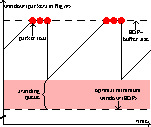
\includegraphics[height=0.9\textheight,keepaspectratio]{figures/cocoa_illustration_too_much.pdf}
\end{frame}

\begin{frame}{Buffer too small}
            \centering
  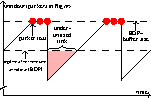
\includegraphics[height=0.9\textheight,keepaspectratio]{figures/cocoa_illustration_too_little.pdf}
\end{frame}

\begin{frame}{Buffer perfect}
            \centering
  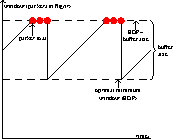
\includegraphics[height=0.9\textheight,keepaspectratio]{figures/cocoa_illustration_perfect.pdf}
\end{frame}

\begin{frame}{\texttt{cocoa} qdisc\footnote{\textit{Cocoa: Congestion Control Aware Queuing}, Bachl, Fabini, Zseby, 2020}}
\begin{itemize}
\item Fair queuing-based qdisc which \textbf{adapts} buffer \textbf{depending on congestion control}
\item Manages to achieve optimal throughput while keeping \textbf{delay} from buffering \textbf{minimal}
\item \textbf{Works} for common congestion controls
\end{itemize}
\pause
\begin{alertblock}{Hand-crafted algorithm:}
Works well for current congestion controls but might fail badly for new congestion controls.
\end{alertblock}
\end{frame}

\section{Concept}

\begin{frame}{Deep Learning for Buffering}
\begin{itemize}
\item Define some objective (like high throughput, low delay)
\item Use Deep Learning to learn the optimal buffering policy for each flow
\end{itemize}
\end{frame}

\begin{frame}{Objective}
\begin{align*}
\textit{Objective} = \textit{bandwidth}-\alpha\times\textit{queue size}
\end{align*}
\end{frame}

\begin{frame}{Input features}
\begin{itemize}
\item queue size
\item standard deviation of the queue size 
\item maximimum allowed buffer size
\item rate of incoming data
\item rate of outgoing data
\item time since the last packet loss
\end{itemize}
\end{frame}

\begin{frame}{Input features 2}
\begin{itemize}
\item Don't use these features themselves but exponentially weighted moving averages
\item Advantage: No need to keep data around except for features themselves
\end{itemize}
\end{frame}

\begin{frame}{Neural Network}
\begin{itemize}
\item Fully connected neural network with three layers and leaky ReLU
\item Outputs optimal maximum buffer size each time packet is received
\item This makes it a regression problem
\end{itemize}
\end{frame}

\begin{frame}{Offline Learning}
\begin{itemize}
\item Randomly sample bandwidth, delay, congestion control and flow duration
\item For each flow, at random time, launch experiment
\item Experiment is A/B testing: 
\begin{itemize}
\item Continue with current buffer size +1 and current buffer size -1 (two different experiment)
\item Let the neural network learn buffer size that performed better regarding objective
\end{itemize}
\item Train using L1 loss (mean absolute error) and batch size of 20
\end{itemize}
\end{frame}

\begin{frame}{Online Learning}
Same as Offline Learning except:
\begin{itemize}
\item Don't do A/B testing
\item Instead: Use second neural network that outputs expected objective function (trained using L2 loss (mean squared error).
\item Either perform experiment A \textbf{or} experiment B
\item If result was better than expected by second neural network, let first neural network learn to output this buffer size in the future.
\end{itemize}
\end{frame}

\section{Results}

%\includegraphics[width=0.98\columnwidth]{{"../ns-allinone-3.30.1/ns-3.30.1/results/RLQueueDisc/logs/plots/2020-6-6-10-24-18_81000.weights_New Reno_bandwidth"}.pdf}
%}{}
%\subfloat[New Reno, varying delay.\label{fig:SmallAlphaNewRenoDelay}
%]{
%\includegraphics[width=0.98\columnwidth]{{"../ns-allinone-3.30.1/ns-3.30.1/results/RLQueueDisc/logs/plots/2020-6-6-10-24-18_81000.weights_New Reno_delay"}.pdf}
%}{}
%\subfloat[BIC, varying bandwidth\label{fig:SmallAlphaBicBandwidth}
%]{
%\includegraphics[width=0.98\columnwidth]{{"../ns-allinone-3.30.1/ns-3.30.1/results/RLQueueDisc/logs/plots/2020-6-6-10-24-18_81000.weights_Bic_bandwidth"}.pdf}
%}{}
%\subfloat[BIC, varying delay\label{fig:SmallAlphaBicDelay}
%]{
%\includegraphics[width=0.98\columnwidth]{{"../ns-allinone-3.30.1/ns-3.30.1/results/RLQueueDisc/logs/plots/2020-6-6-10-24-18_81000.weights_Bic_delay"}.pdf}
%}{}

\begin{frame}{Offline, $\alpha = 0.01$, New Reno}
\centering
\includegraphics[width=0.9\columnwidth]{{"../ns-allinone-3.30.1/ns-3.30.1/results/RLQueueDisc/logs/plots/2020-6-6-10-24-18_81000.weights_New Reno_bandwidth"}.pdf}
\end{frame}

\begin{frame}{Offline, $\alpha = 0.01$, New Reno}
\centering
\includegraphics[width=0.9\columnwidth]{{"../ns-allinone-3.30.1/ns-3.30.1/results/RLQueueDisc/logs/plots/2020-6-6-10-24-18_81000.weights_New Reno_delay"}.pdf}
\end{frame}

\begin{frame}{Offline, $\alpha = 0.01$, Bic}
\centering
\includegraphics[width=0.9\columnwidth]{{"../ns-allinone-3.30.1/ns-3.30.1/results/RLQueueDisc/logs/plots/2020-6-6-10-24-18_81000.weights_Bic_bandwidth"}.pdf}
\end{frame}

\begin{frame}{Offline, $\alpha = 0.01$, Bic}
\centering
\includegraphics[width=0.9\columnwidth]{{"../ns-allinone-3.30.1/ns-3.30.1/results/RLQueueDisc/logs/plots/2020-6-6-10-24-18_81000.weights_Bic_delay"}.pdf}
\end{frame}

\begin{frame}{Offline training progress}
\begin{figure}[h]
\includegraphics[width=0.9\columnwidth]{/mnt/cluster/results/RLQueueDisc/logs/plots/2020-6-4-15-39-25_prediction.png}
\end{figure}
\end{frame}

\begin{frame}{Online training progress}
\begin{figure}[h]
\includegraphics[width=0.9\columnwidth]{/mnt/cluster/results/RLQueueDisc/logs/plots/2020-6-1-16-41-30_prediction.png}
\end{figure}
\end{frame}

\begin{frame}{Example: Queue size with our solution}
\begin{figure}[h]
\includegraphics[width=0.9\columnwidth]{{"../ns-allinone-3.30.1/ns-3.30.1/results/RLQueueDisc/queueTraces/2020-6-6-10-24-18_81000.weights/cc_0_bw_15.000000_delay_5.606061_queue"}.pdf}
\end{figure}
\end{frame}

\begin{frame}{Example flow: Queue size with FqCoDel (default on home routers)}
\begin{figure}[h]
\includegraphics[width=0.9\columnwidth]{{"../ns-allinone-3.30.1/ns-3.30.1/results/FqCoDelQueueDisc/queueTraces/cc_0_bw_15.000000_delay_5.606061_queue"}.pdf}
\end{figure}
\end{frame}

\begin{frame}{Example flow: Queue size with Fifo (default on Linux)}
\begin{figure}[h]
\includegraphics[width=0.9\columnwidth]{{"../ns-allinone-3.30.1/ns-3.30.1/results/FifoQueueDisc/queueTraces/cc_0_bw_15.000000_delay_5.606061_queue"}.pdf}
\end{figure}
\end{frame}

\section{Discussion}

\begin{frame}{What works}
\begin{itemize}
\item Learns the objective successfully
\item Behavior makes more sense than that of competing solutions
\item Low computational overhead
\end{itemize}
\end{frame}

\begin{frame}{What could be improved}
\begin{itemize}
\item Behavior seems unstable sometimes
\begin{itemize}
\item Maybe lower training rate?
\item Not L1 loss (mean absolute error) but L2 loss (mean squared error)? 
\end{itemize}
\item Online learning doesn't work for small $\alpha$. But is this really a problem?
\end{itemize}
\end{frame}

% -------------
% Last page
% -------------
\makelastslide

\end{document}